\chapter{Cryptographic Primitives}

In this chapter, we examine how cryptographic primitives are integrated and how the abstraction layer orchestrates with key generation, hashing, and digital signature operations.
\begin{center}
\begin{minipage}{.49\textwidth}
\begin{verbatim}
CryptoModule/
├─ include
│ └─ crypto
│     ├─ cryptoarith.h
│     ├─ crypto_ecc_config.h
│     ├─ crypto_ecc_types.h
│     ├─ cryptoec.h
│     ├─ cryptosig.h
│     ├─ curves
│     │ ├─ aff_pt.h
│     │ ├─ curves.h
│     │ ├─ curves_list.h
│     │ ├─ ec_params_external.h
│     │ ├─ ec_params.h
│     │ ├─ ec_params_secp256r1.h
│     │ ├─ ec_shortw.h
│     │ └─ prj_pt.h
│     ├─ external_deps
│     │ ├─ print.h
│     │ ├─ rand.h
│     │ └─ time.h
│     ├─ fp
│     │ ├─ fp_add.h
│     │ ├─ fp_config.h
│     │ ├─ fp.h
│     │ ├─ fp_montgomery.h
│     │ ├─ fp_mul.h
│     │ ├─ fp_mul_redc1.h
│     │ ├─ fp_pow.h
│     │ ├─ fp_rand.h
│     │ └─ fp_sqrt.h
\end{verbatim}
\end{minipage}
\begin{minipage}{.49\textwidth}
\begin{verbatim}
│     ├─ hash
│     │ ├─ hash_algs.h
│     │ ├─ hmac.h
│     │ ├─ keccak.h
│     │ ├─ sha256.h
│     │ ├─ sha2.h
│     │ ├─ sha3-256.h
│     │ ├─ sha3.h
│     │ ├─ shake256.h
│     │ └─ shake.h
│     ├─ nn
│     │ ├─ nn_add.h
│     │ ├─ nn_config.h
│     │ ├─ nn_div.h
│     │ ├─ nn_div_public.h
│     │ ├─ nn.h
│     │ ├─ nn_logical.h
│     │ ├─ nn_modinv.h
│     │ ├─ nn_mod_pow.h
│     │ ├─ nn_mul.h
│     │ ├─ nn_mul_public.h
│     │ ├─ nn_mul_redc1.h
│     │ └─ nn_rand.h
│     ├─ sig
│     │ ├─ ecdsa_common.h
│     │ ├─ ecdsa.h
│     │ ├─ ec_key.h
│     │ ├─ sig_algs.h
│     │ └─ sig_algs_internal.h
│     ├─ utils
│     │ ├─ ...
│     └─ words
│     │ ├─ ..
\end{verbatim}
\end{minipage}
\end{center}

\newpage

\section{Overview of Libraries}
A key feature of the library is its use of an abstraction layer to support multiple cryptographic algorithms through a unified interface.
\begin{figure}[h!]
	\centering
	\begin{tikzpicture}[
		% Define styles for the nodes and layers
		layer_box/.style={
			rectangle, 
			draw, 
			thick, 
			fill=blue!5, 
			text width=0.95\textwidth, 
			minimum height=3.5cm, 
			align=left,
			rounded corners=5pt,
			drop shadow={opacity=0.5}
		},
		app_node/.style={
			rectangle, 
			draw, 
			thick,
			fill=green!15, 
			text centered,
			font=\sffamily,
			minimum height=1cm,
			rounded corners=3pt
		},
		data_node/.style={
			trapezium, 
			trapezium left angle=70, 
			trapezium right angle=110,
			draw, 
			thick,
			fill=orange!20,
			text centered,
			font=\sffamily,
			minimum height=1cm,
			drop shadow
		},
		arrow_style/.style={
			-latex, 
			thick,
			draw=black!70
		},
		]
		
		% ----- Nodes -----
		% Define the three main layers
		\node[layer_box] (crypto_layer) at (0, -9) {};
		\node[] at (-4.6, -7) {\textbf{Cryptographic Primitives Layer}};
		
		% Components for the Cryptographic Primitives Layer
		\node[app_node, fill=blue!20, text width=10cm, align=center] (libecc) at (0, -9) {\textbf{Core Library}\\ (\texttt{libarith.a}, \texttt{libec.a}, \texttt{libsig.a})};
		%		\node[font=\sffamily\small] at (0, -9.25) {};

			
	\end{tikzpicture}
	\caption{\textbf{Cryptographic Primitive Layer.}\; This is a low-level cryptographic operations includes three libraries: \texttt{libarith.a}, \texttt{libec.a}, \texttt{libsig.a}.}
	\label{fig:architecture}
\end{figure}

\begin{center}
\begin{minipage}{.475\textwidth}
\paragraph{libarith.a}\ \\
\begin{lstlisting}[style=cstyle, caption={include/cryptoarith.h}, captionpos=t]
#ifndef __CRYPTOARITH_H__
#define __CRYPTOARITH_H__
/* NN layer includes */
#include <crypto/nn/nn.h>
#include <crypto/nn/nn_logical.h>
#include <crypto/nn/nn_add.h>
#include <crypto/nn/nn_mul_public.h>
#include <crypto/nn/nn_mul_redc1.h>
#include <crypto/nn/nn_div_public.h>
#include <crypto/nn/nn_modinv.h>
#include <crypto/nn/nn_mod_pow.h>
#include <crypto/nn/nn_rand.h>
#include <crypto/utils/print_nn.h>
/* Fp layer include */
#include <crypto/fp/fp.h>
#include <crypto/fp/fp_add.h>
#include <crypto/fp/fp_montgomery.h>
#include <crypto/fp/fp_mul.h>
#include <crypto/fp/fp_sqrt.h>
#include <crypto/fp/fp_pow.h>
#include <crypto/fp/fp_rand.h>
#include <crypto/utils/print_fp.h>
\end{lstlisting}
\end{minipage}\hfill
\begin{minipage}{.475\textwidth}
\paragraph{libec.a}\ \\
\begin{lstlisting}[style=cstyle, caption={include/cryptoec.h}, captionpos=t]
#ifndef __CRYPTOEC_H__
#define __CRYPTOEC_H__
/* Include the cryptoarith package */
#include <crypto/cryptoarith.h>
/* Curve layer includes */
#include <crypto/curves/curves.h>
#include <crypto/curves/curves_list.h>
#include <crypto/curves/ec_shortw.h>
#include <crypto/curves/prj_pt.h>
#include <crypto/curves/aff_pt.h>
#include <crypto/utils/print_curves.h>
#endif /* __CRYPTOEC_H__ */
\end{lstlisting}
\paragraph{libsig.a}\ \\
\begin{lstlisting}[style=cstyle, caption={include/cryptosig.h}, captionpos=t]
#ifndef __CRYPTOSIG_H__
#define __CRYPTOSIG_H__
/* Include the Elliptic Curves layer */
#include <crypto/cryptoec.h>
#include <crypto/crypto_ecc_config.h>
#include <crypto/crypto_ecc_types.h>
#include <crypto/sig/sig_algs.h>
#include <crypto/sig/ec_key.h>
#include <crypto/utils/dbg_sig.h>
/* Include the hash functions */
#include <crypto/hash/hash_algs.h>
/* Include the hmac functions */
#include <crypto/hash/hmac.h>
#endif /* __CRYPTOSIG_H__ */
\end{lstlisting}
\end{minipage}
\end{center}

\newpage
\section{Modular Arithmetic and Finite Field Library}
\begin{figure}[h!]\centering
	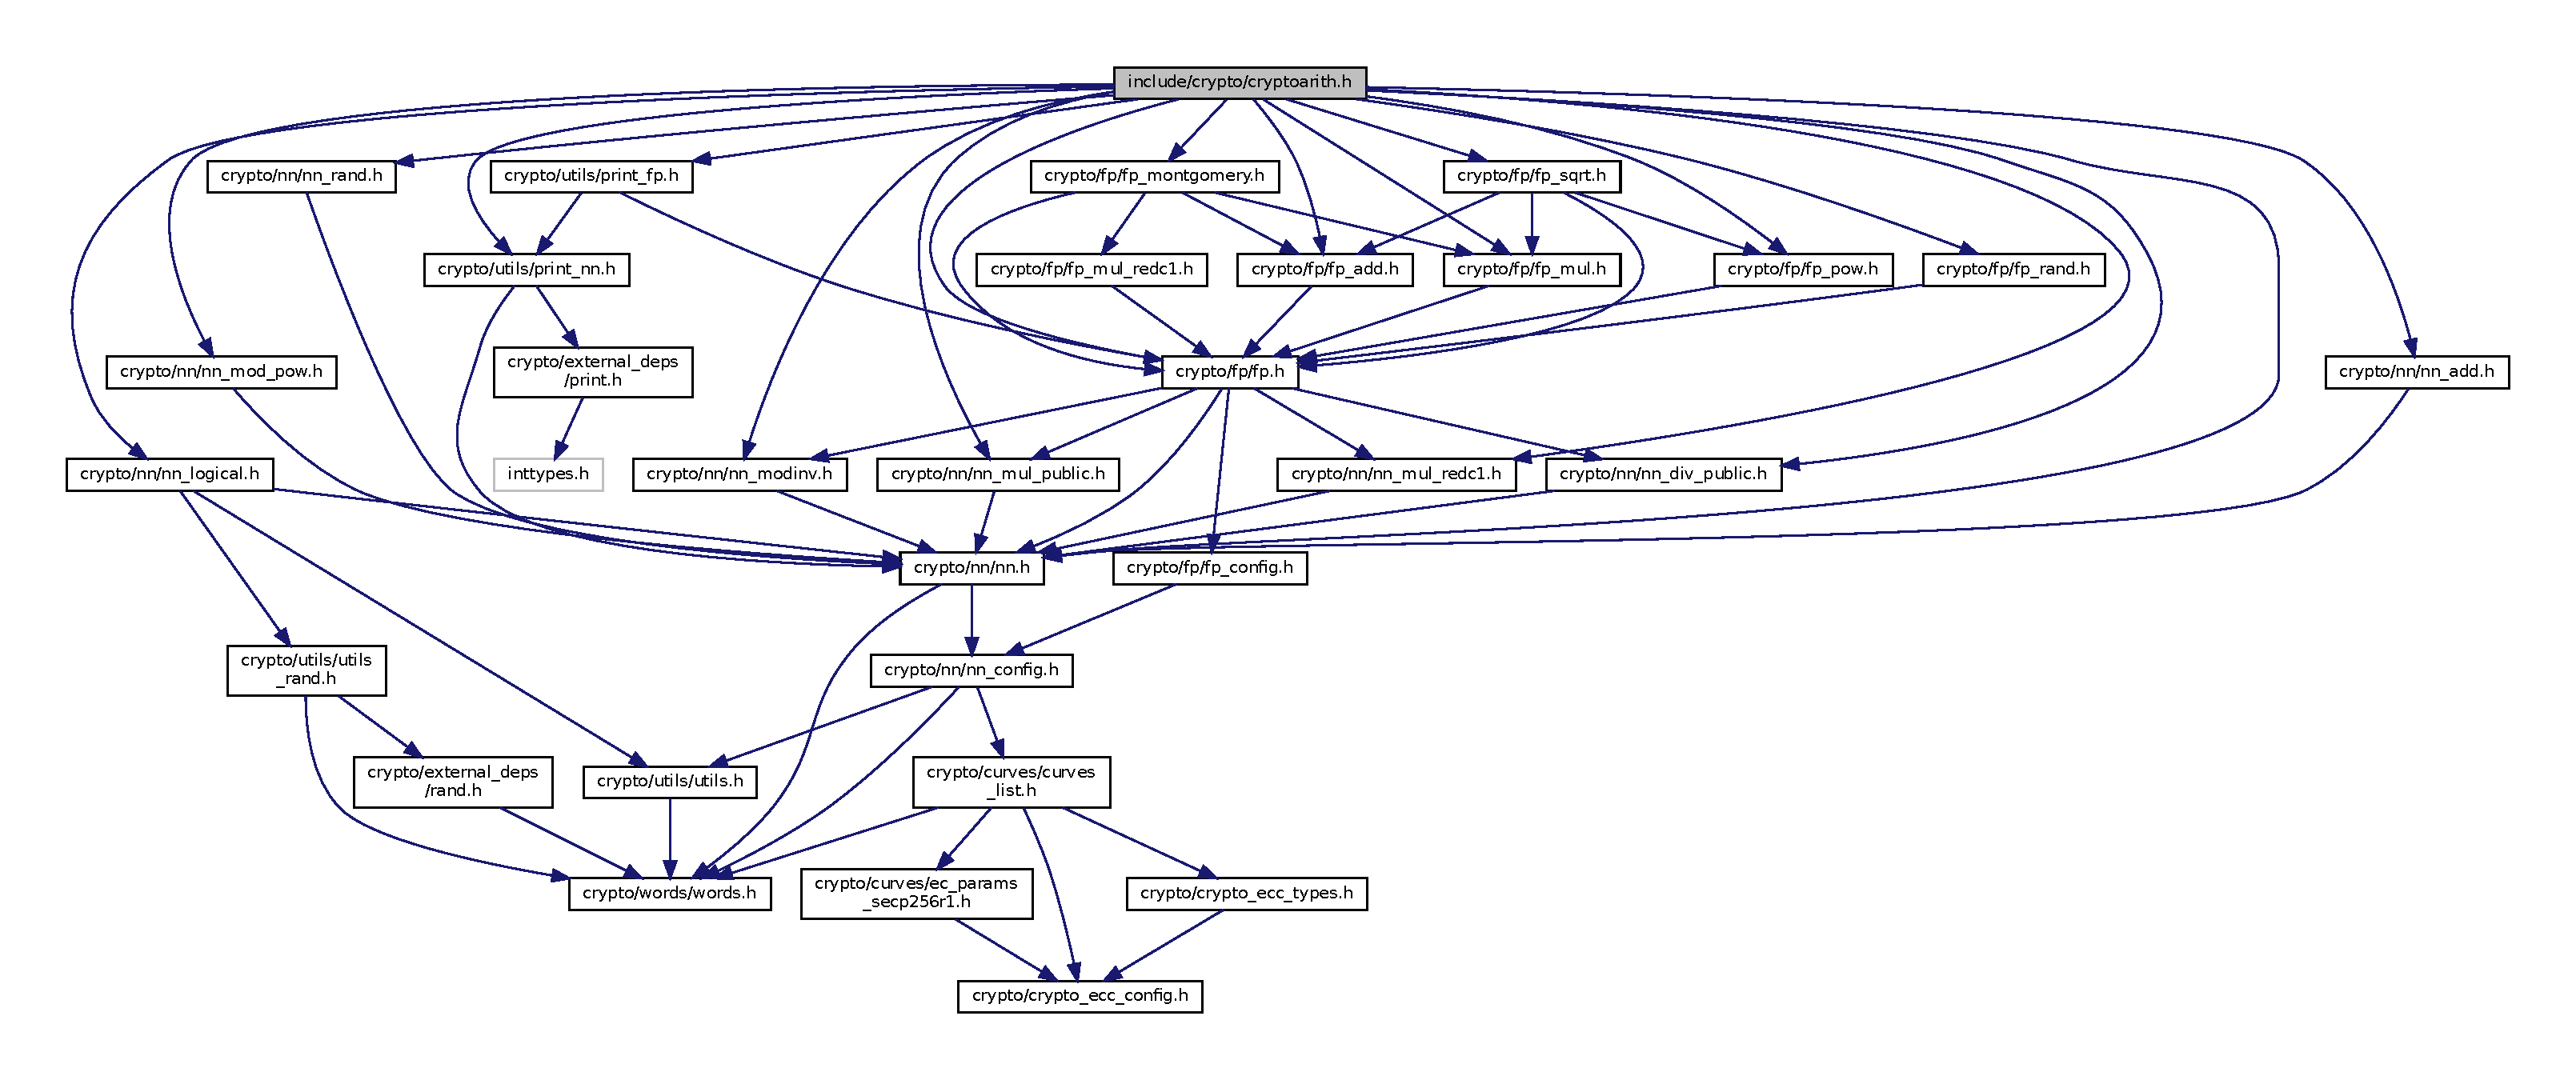
\includegraphics[scale=.4265, angle=-90]{dep-graph/cryptoarith.pdf}
\end{figure}
\newpage
\subsection{Modular Arithmetic}
\begin{figure}[h!]\centering
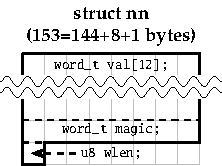
\includegraphics[scale=2.15]{struct-tikz/nn.pdf}
\end{figure}
\begin{lstlisting}[style=cstyle, caption={include/nn/nn.h}, captionpos=t]
#ifndef __NN_H__
#define __NN_H__

#include <crypto/words/words.h>
#include <crypto/nn/nn_config.h>

typedef struct {
	word_t val[BIT_LEN_WORDS(NN_MAX_BIT_LEN)];
	word_t magic;
	u8 wlen;
} nn;

typedef nn *nn_t;
typedef const nn *nn_src_t;

int nn_check_initialized(nn_src_t A);
int nn_is_initialized(nn_src_t A);
int nn_zero(nn_t A);
int nn_one(nn_t A);
int nn_set_word_value(nn_t A, word_t val);
void nn_uninit(nn_t A);
int nn_init(nn_t A, u16 len);
int nn_init_from_buf(nn_t A, const u8 *buf, u16 buflen);
int nn_cnd_swap(int cnd, nn_t in1, nn_t in2);
int nn_set_wlen(nn_t A, u8 new_wlen);
int nn_iszero(nn_src_t A, int *iszero);
int nn_isone(nn_src_t A, int *isone);
int nn_isodd(nn_src_t A, int *isodd);
int nn_cmp_word(nn_src_t in, word_t w, int *cmp);
int nn_cmp(nn_src_t A, nn_src_t B, int *cmp);
int nn_copy(nn_t dst_nn, nn_src_t src_nn);
int nn_normalize(nn_t in1);
int nn_export_to_buf(u8 *buf, u16 buflen, nn_src_t in_nn);
int nn_tabselect(nn_t out, u8 idx, nn_src_t *tab, u8 tabsize);

#endif /* __NN_H__ */
\end{lstlisting}

\newpage
\subsection{Finite Field}
\begin{figure}[h!]\centering
	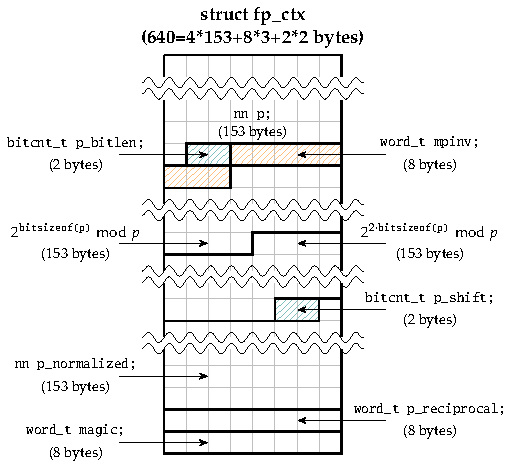
\includegraphics[scale=1.25]{struct-tikz/fp_ctx.pdf}
\end{figure}
\begin{lstlisting}[style=cstyle, caption={include/fp/fp.h}, captionpos=t]
#ifndef __FP_H__
#define __FP_H__

#include <crypto/nn/nn.h>
#include <crypto/nn/nn_div_public.h>
#include <crypto/nn/nn_modinv.h>
#include <crypto/nn/nn_mul_public.h>
#include <crypto/nn/nn_mul_redc1.h>
#include <crypto/fp/fp_config.h>

typedef struct {
	/*
	* Value of p (extended by one word to handle overflows in Fp). 
	* p_bitlen provides its length in bit.
	*/
	nn p;
	bitcnt_t p_bitlen;
	
	word_t mpinv;	/* -p^-1 mod 2^(bitsizeof(word_t)) */
	nn r;	/* 2^bitsizeof(p) mod p */
	nn r_square;	/* 2^(2*bitsizeof(p)) mod p */

	bitcnt_t p_shift;		/* clz(p) */
	nn p_normalized;	/* p << p_shift */
	word_t p_reciprocal;	/* floor(B^3/(DMSW(p_normalized) + 1)) - B */
	
	word_t magic;
} fp_ctx;

typedef fp_ctx *fp_ctx_t;
typedef const fp_ctx *fp_ctx_src_t;

int fp_ctx_check_initialized(fp_ctx_src_t ctx);
int fp_ctx_init(fp_ctx_t ctx, nn_src_t p, bitcnt_t p_bitlen, nn_src_t r, nn_src_t r_square, word_t mpinv, bitcnt_t p_shift, nn_src_t p_normalized, word_t p_reciprocal);
int fp_ctx_init_from_p(fp_ctx_t ctx, nn_src_t p);

/* Then the definition of our Fp elements */
typedef struct {
	nn fp_val;
	fp_ctx_src_t ctx;
	word_t magic;
} fp;

typedef fp *fp_t;
typedef const fp *fp_src_t;

int fp_check_initialized(fp_src_t in);
int fp_init(fp_t A, fp_ctx_src_t fpctx);
int fp_init_from_buf(fp_t A, fp_ctx_src_t fpctx, const u8 *buf, u16 buflen);
void fp_uninit(fp_t A);
int fp_set_nn(fp_t out, nn_src_t in);
int fp_zero(fp_t out);
int fp_one(fp_t out);
int fp_set_word_value(fp_t out, word_t val);
int fp_cmp(fp_src_t in1, fp_src_t in2, int *cmp);
int fp_iszero(fp_src_t in, int *iszero);
int fp_copy(fp_t out, fp_src_t in);
int fp_tabselect(fp_t out, u8 idx, fp_src_t *tab, u8 tabsize);
int fp_eq_or_opp(fp_src_t in1, fp_src_t in2, int *eq_or_opp);
int fp_import_from_buf(fp_t out_fp, const u8 *buf, u16 buflen);
int fp_export_to_buf(u8 *buf, u16 buflen, fp_src_t in_fp);

#endif /* __FP_H__ */
\end{lstlisting}

\begin{figure}[h!]\centering
	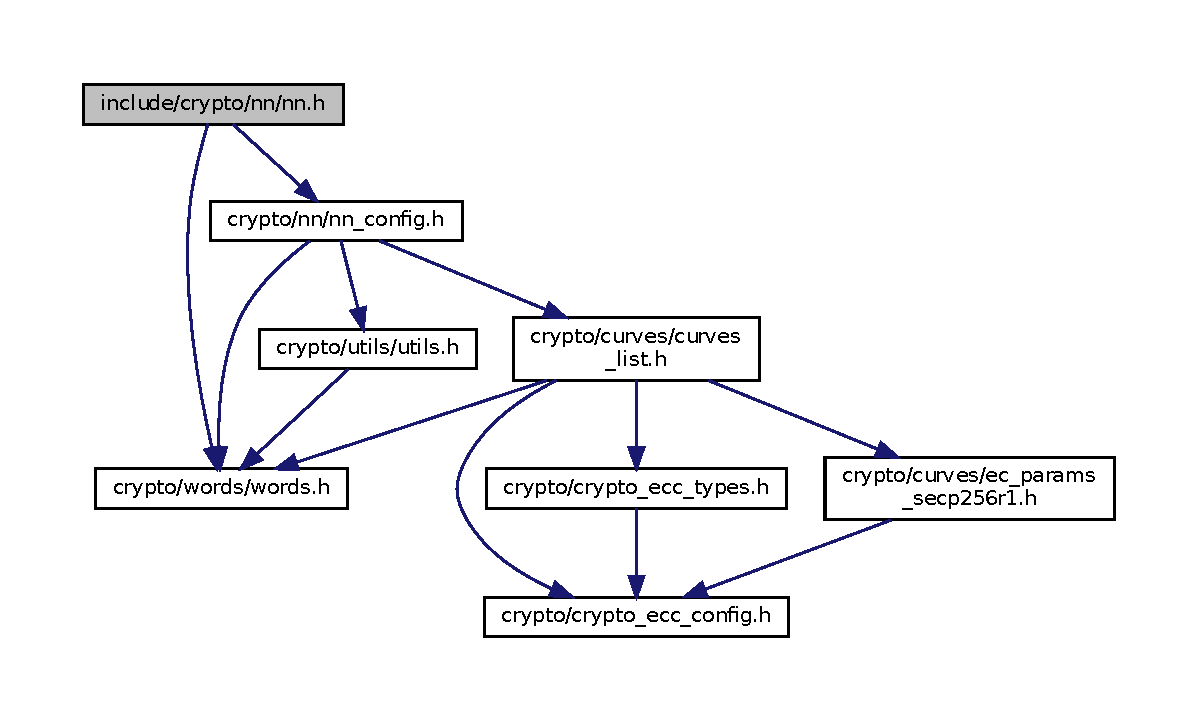
\includegraphics[scale=.7]{dep-graph/nn.pdf}
\end{figure}

\newpage
\section{Elliptic Curve Library}
\begin{figure}[h!]\centering
	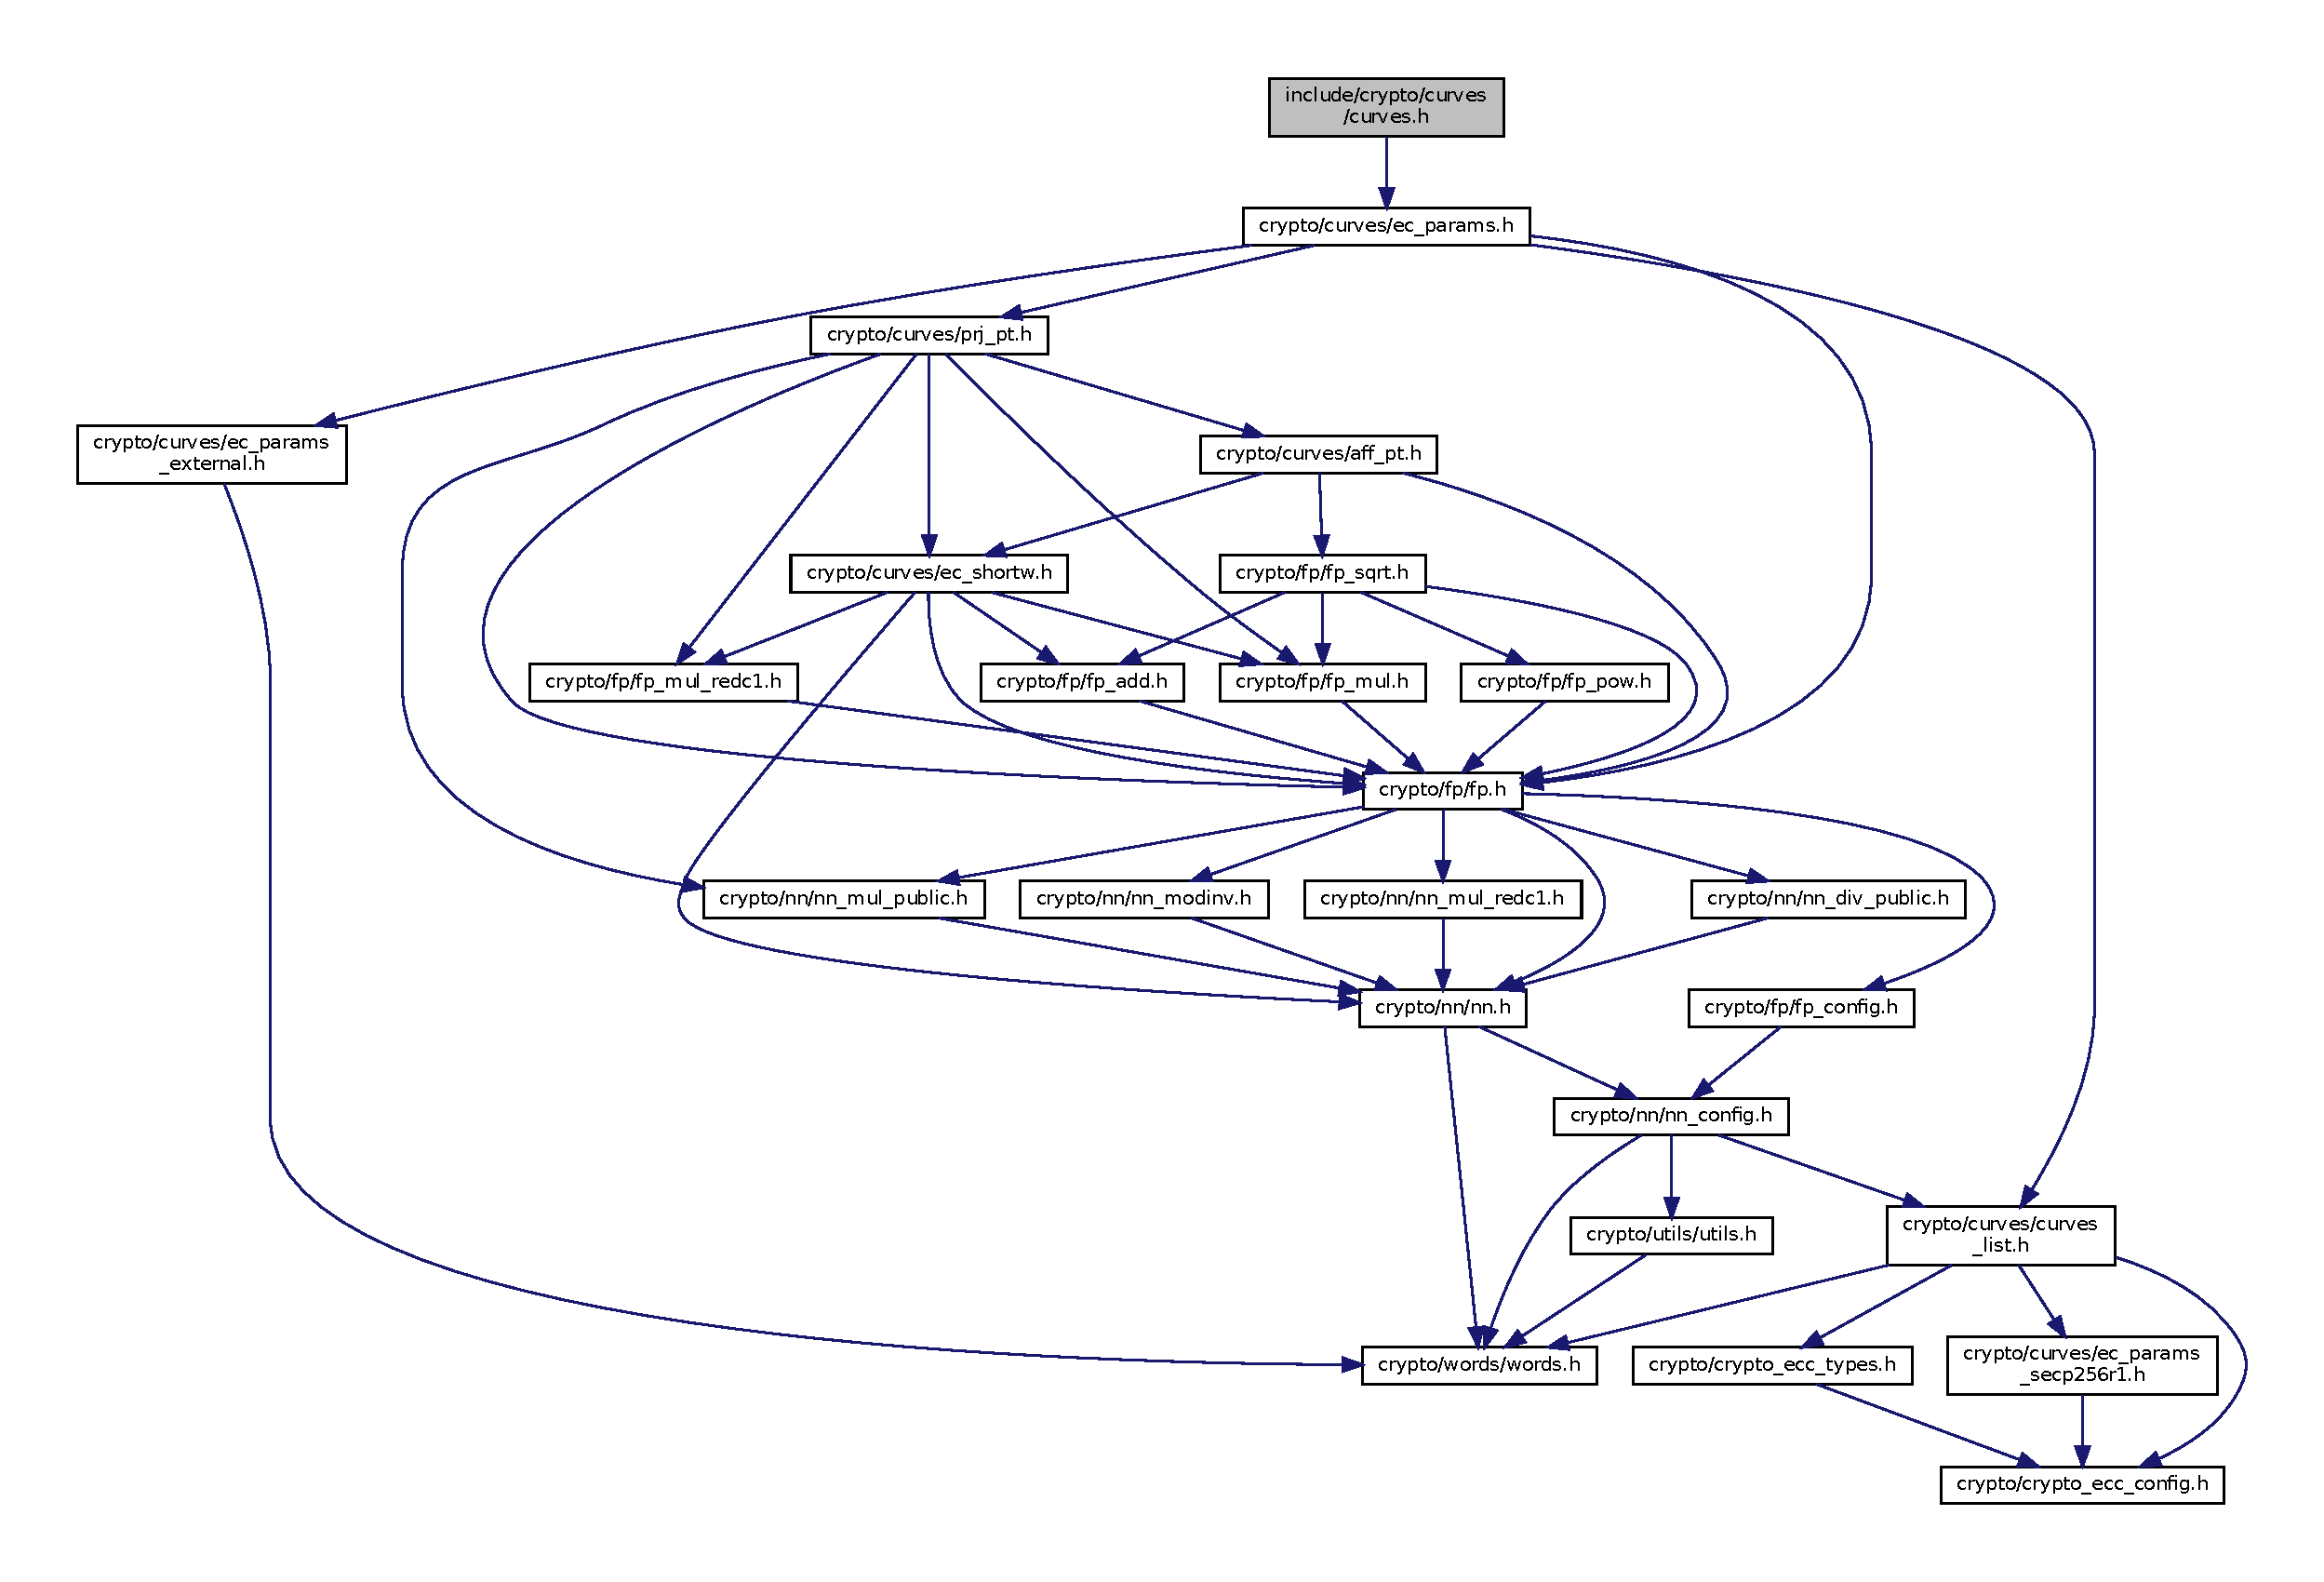
\includegraphics[scale=.545, angle=-90]{dep-graph/curves.pdf}
\end{figure}
\newpage
\subsection{Short Weierstrass Form}
\begin{lstlisting}[style=cstyle, caption={include/curves/ec\_shortw.h}, captionpos=t]
#ifndef __EC_SHORTW_H__
#define __EC_SHORTW_H__

#include <crypto/nn/nn.h>
#include <crypto/fp/fp.h>
#include <crypto/fp/fp_add.h>
#include <crypto/fp/fp_mul.h>
#include <crypto/fp/fp_mul_redc1.h>

typedef struct {
	fp a; fp b; fp a_monty;
#ifndef NO_USE_COMPLETE_FORMULAS
	fp b3; fp b_monty; fp b3_monty;
#endif
	nn order; /* curve order */
	word_t magic;
} ec_shortw_crv;

typedef ec_shortw_crv *ec_shortw_crv_t;
typedef const ec_shortw_crv *ec_shortw_crv_src_t;

int ec_shortw_crv_check_initialized(ec_shortw_crv_src_t crv);
int ec_shortw_crv_init(ec_shortw_crv_t crv, fp_src_t a, fp_src_t b, nn_src_t order);
void ec_shortw_crv_uninit(ec_shortw_crv_t crv);

#endif /* __EC_SHORTW_H__ */
\end{lstlisting}
\begin{figure}[h!]\centering
	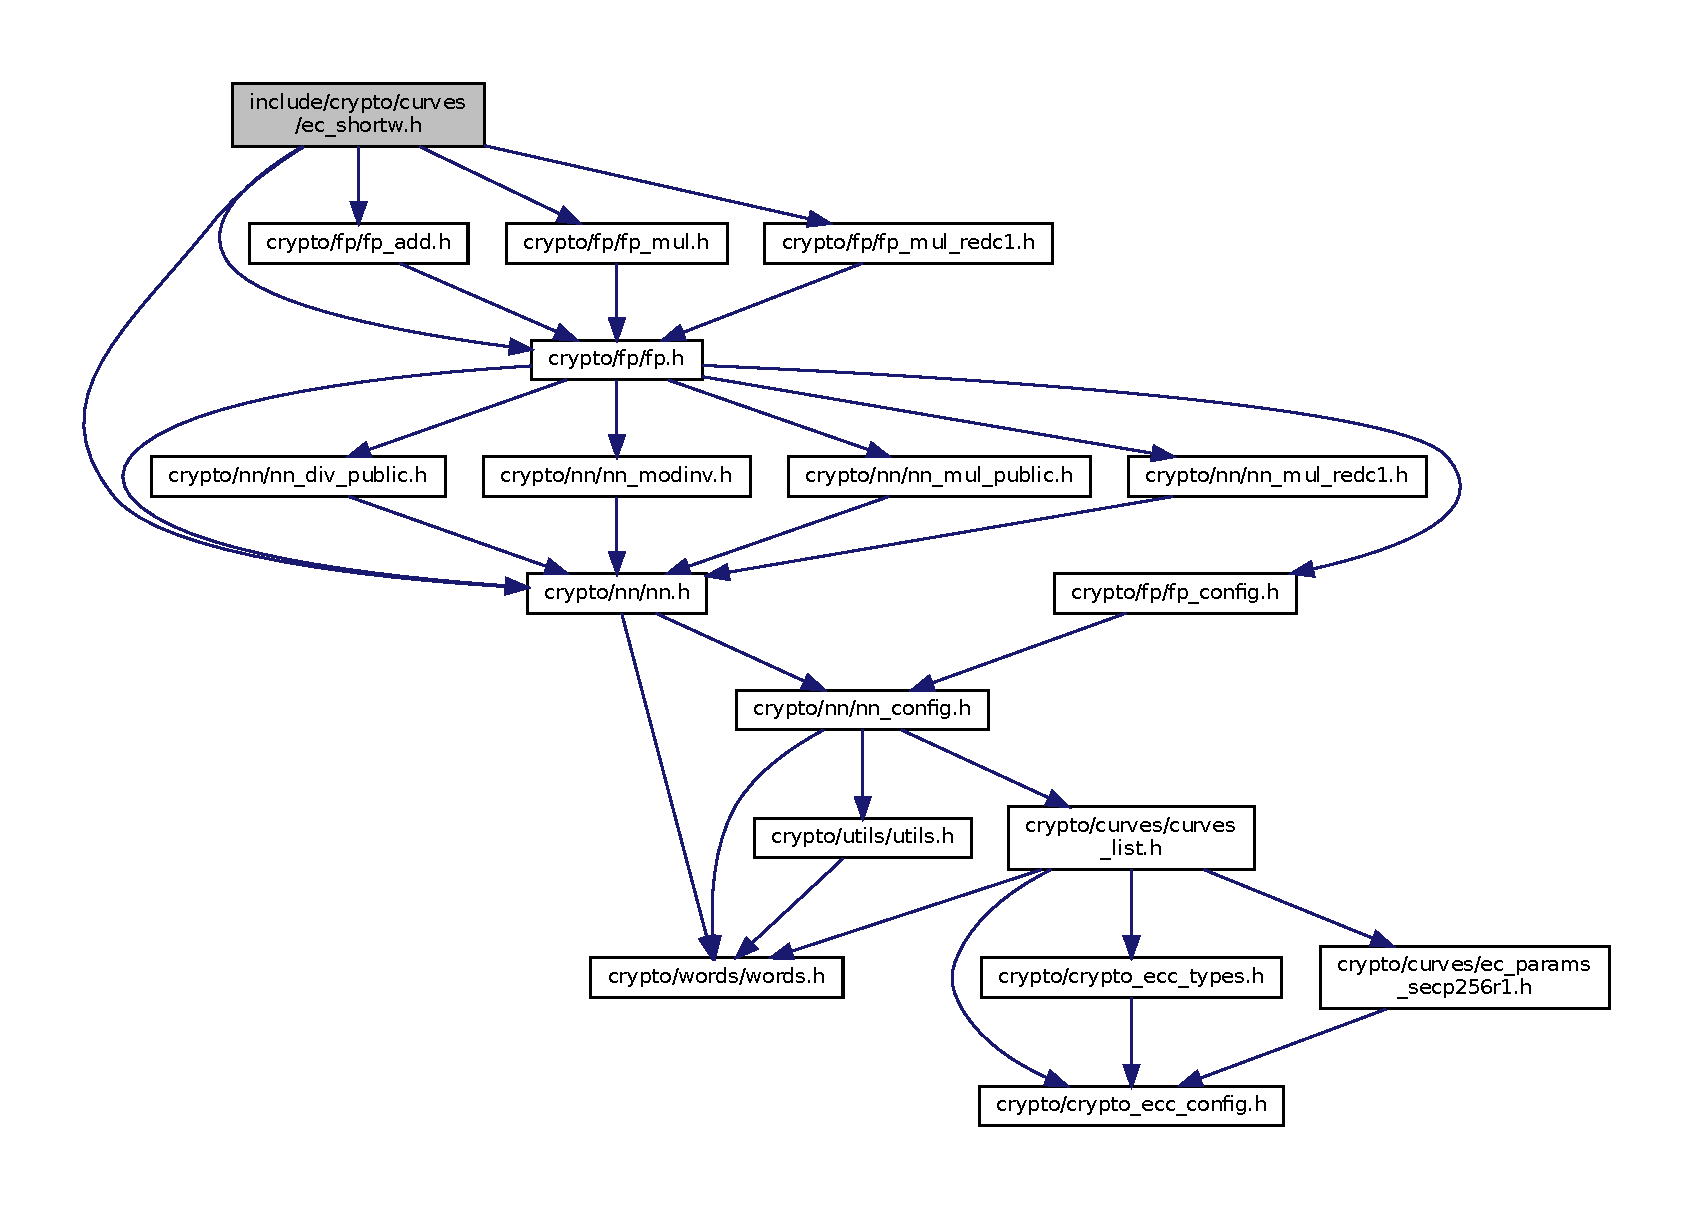
\includegraphics[scale=.545]{dep-graph/ec_shortw.pdf}
\end{figure}

\newpage
\subsection{Points of Affine Coordinate}
\begin{lstlisting}[style=cstyle, caption={include/curves/aff\_pt.h}, captionpos=t]
#ifndef __AFF_PT_H__
#define __AFF_PT_H__
#include <crypto/fp/fp.h>
#include <crypto/fp/fp_sqrt.h>
#include <crypto/curves/ec_shortw.h>
typedef struct {
	fp x; fp y; 
	ec_shortw_crv_src_t crv;
	word_t magic;
} aff_pt;
typedef aff_pt *aff_pt_t;
typedef const aff_pt_t aff_pt_src_t;
int aff_pt_check_initialized(aff_pt_src_t in);
int aff_pt_init(aff_pt_t in, ec_shortw_crv_src_t curve);
int aff_pt_init_from_coords(aff_pt_t in, ec_shortw_crv_src_t curve, fp_src_t xcoord, fp_src_t ycoord);
void aff_pt_uninit(aff_pt_t in);
int aff_pt_y_from_x(fp_t y1, fp_t y2, fp_src_t x, ec_shortw_crv_src_t curve);
int is_on_shortw_curve(fp_src_t x, fp_src_t y, ec_shortw_crv_src_t curve, int *on_curve);
int aff_pt_is_on_curve(aff_pt_src_t pt, int *on_curve);
int ec_shortw_aff_copy(aff_pt_t out, aff_pt_src_t in);
int ec_shortw_aff_cmp(aff_pt_src_t in1, aff_pt_src_t in2, int *cmp);
int ec_shortw_aff_eq_or_opp(aff_pt_src_t in1, aff_pt_src_t in2, int *eq_or_opp);
int aff_pt_import_from_buf(aff_pt_t pt, const u8 *pt_buf, u16 pt_buf_len, ec_shortw_crv_src_t crv);
int aff_pt_export_to_buf(aff_pt_src_t pt, u8 *pt_buf, u32 pt_buf_len);
#endif /* __AFF_PT_H__ */

\end{lstlisting}
\begin{figure}[h!]\centering
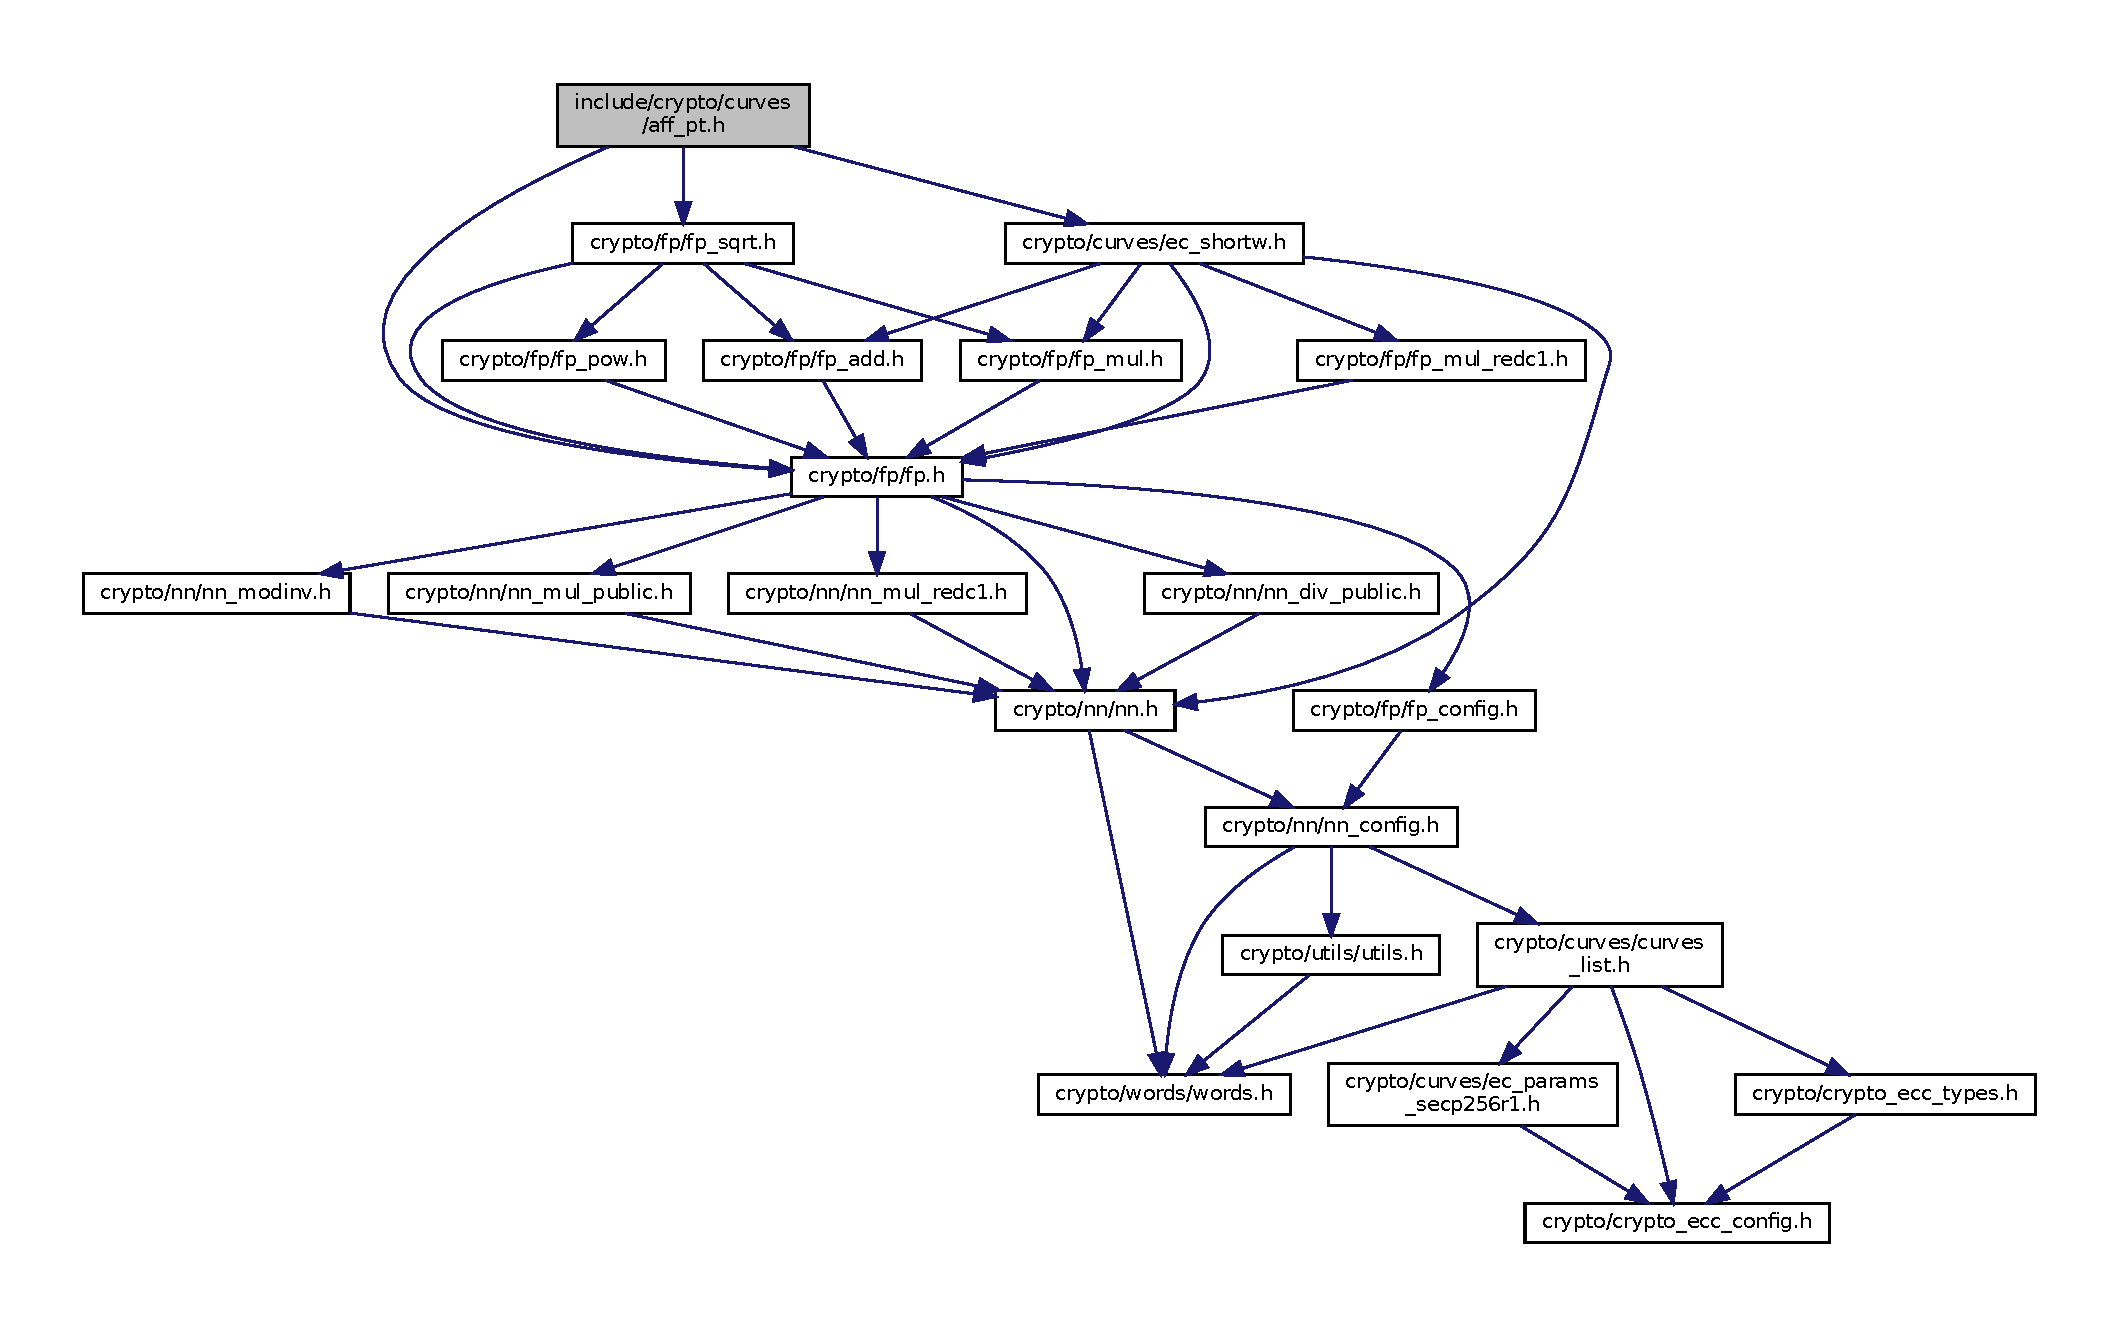
\includegraphics[scale=.45]{dep-graph/aff_pt.pdf}
\end{figure}
\newpage

\subsection{Points of Projective Coordinate}
\begin{lstlisting}[style=cstyle, caption={include/curves/prj\_pt.h}, captionpos=t]
#ifndef __PRJ_PT_H__
#define __PRJ_PT_H__

#include <crypto/nn/nn_mul_public.h>
#include <crypto/fp/fp.h>
#include <crypto/fp/fp_mul.h>
#include <crypto/fp/fp_mul_redc1.h>
#include <crypto/curves/ec_shortw.h>
#include <crypto/curves/aff_pt.h>

typedef struct {
	fp X; fp Y; fp Z;
	ec_shortw_crv_src_t crv;
	word_t magic;
} prj_pt;

typedef prj_pt *prj_pt_t;
typedef const prj_pt *prj_pt_src_t;
typedef enum {
	PUBLIC_PT = 0,
	PRIVATE_PT = 1
} prj_pt_sensitivity;

int prj_pt_check_initialized(prj_pt_src_t in);
int prj_pt_init(prj_pt_t in, ec_shortw_crv_src_t curve);
int prj_pt_init_from_coords(prj_pt_t in, ec_shortw_crv_src_t curve, fp_src_t xcoord, fp_src_t ycoord, fp_src_t zcoord);
void prj_pt_uninit(prj_pt_t in);
int prj_pt_zero(prj_pt_t out);
int prj_pt_iszero(prj_pt_src_t in, int *iszero);
int prj_pt_is_on_curve(prj_pt_src_t in, int *on_curve);
int prj_pt_copy(prj_pt_t out, prj_pt_src_t in);
int prj_pt_to_aff(aff_pt_t out, prj_pt_src_t in);
int prj_pt_unique(prj_pt_t out, prj_pt_src_t in);
int ec_shortw_aff_to_prj(prj_pt_t out, aff_pt_src_t in);
int prj_pt_cmp(prj_pt_src_t in1, prj_pt_src_t in2, int *cmp);
int prj_pt_eq_or_opp(prj_pt_src_t in1, prj_pt_src_t in2, int *eq_or_opp);
int prj_pt_neg(prj_pt_t out, prj_pt_src_t in);
int prj_pt_add(prj_pt_t sum, prj_pt_src_t in1, prj_pt_src_t in2);
int prj_pt_dbl(prj_pt_t dbl, prj_pt_src_t in);
int prj_pt_mul(prj_pt_t out, nn_src_t m, prj_pt_src_t in);
int prj_pt_mul_blind(prj_pt_t out, nn_src_t m, prj_pt_src_t in);
/* XXX: WARNING: this function must only be used on public points! */
int _prj_pt_unprotected_mult(prj_pt_t out, nn_src_t cofactor, prj_pt_src_t public_in);
int check_prj_pt_order(prj_pt_src_t in_shortw, nn_src_t in_isorder, prj_pt_sensitivity s, int *check);
int prj_pt_import_from_buf(prj_pt_t pt, const u8 *pt_buf, u16 pt_buf_len, ec_shortw_crv_src_t crv);
int prj_pt_import_from_aff_buf(prj_pt_t pt, const u8 *pt_buf, u16 pt_buf_len, ec_shortw_crv_src_t crv);
int prj_pt_export_to_buf(prj_pt_src_t pt, u8 *pt_buf, u32 pt_buf_len);
int prj_pt_export_to_aff_buf(prj_pt_src_t pt, u8 *pt_buf, u32 pt_buf_len);

#endif /* __PRJ_PT_H__ */
\end{lstlisting}
\begin{figure}[h!]\centering
	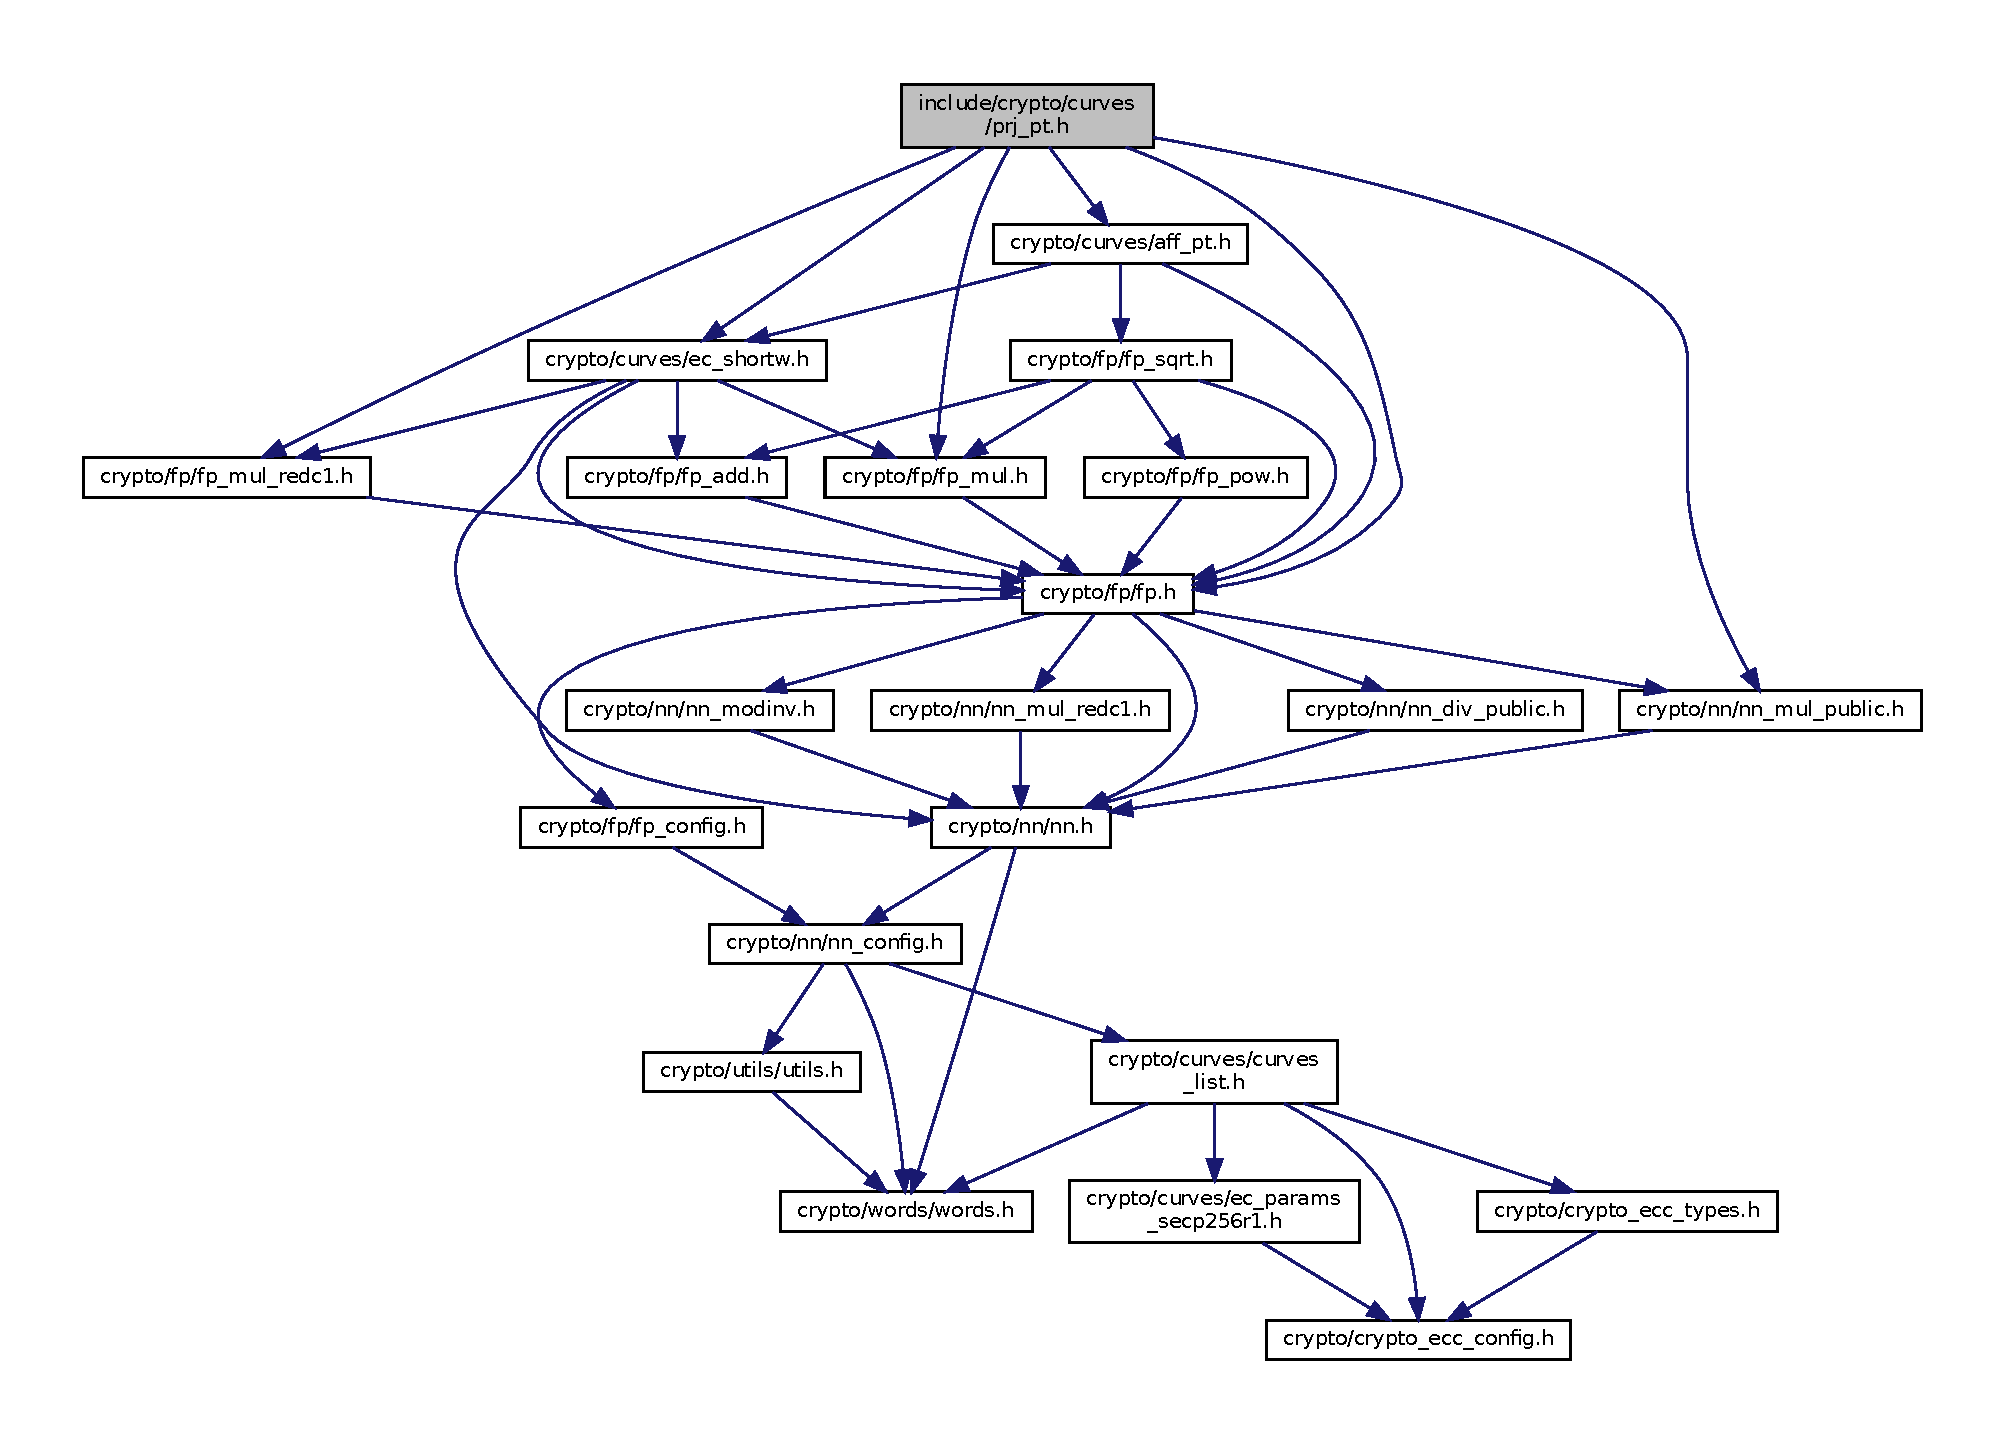
\includegraphics[scale=.675, angle=-90]{dep-graph/prj_pt.pdf}
\end{figure}

\newpage
\ \\
\section{Elliptic Curve Digital Signature Algorithm Library}
\begin{lstlisting}[style=cstyle, caption={include/curves/prj\_pt.h}, captionpos=t]
#include <crypto/crypto_ecc_config.h>
#include <crypto/crypto_ecc_types.h>
#ifndef __ECDSA_COMMON_H__
#define __ECDSA_COMMON_H__

#include <crypto/words/words.h>
#include <crypto/sig/ec_key.h>
#include <crypto/hash/hash_algs.h>
#include <crypto/curves/curves.h>
#include <crypto/utils/utils.h>

#define ECDSA_R_LEN(q_bit_len)  (BYTECEIL(q_bit_len))
#define ECDSA_S_LEN(q_bit_len)  (BYTECEIL(q_bit_len))
#define ECDSA_SIGLEN(q_bit_len) (ECDSA_R_LEN(q_bit_len) + \
ECDSA_S_LEN(q_bit_len))
#define ECDSA_MAX_SIGLEN ECDSA_SIGLEN(CURVES_MAX_Q_BIT_LEN)

/*
* Compute max signature length for all the mechanisms enabled in the library (see lib_ecc_config.h). 
* Having that done during
* preprocessing sadly requires some verbosity.
*/
#ifndef EC_MAX_SIGLEN
#define EC_MAX_SIGLEN 0
#endif
#if ((EC_MAX_SIGLEN) < (ECDSA_MAX_SIGLEN))
#undef EC_MAX_SIGLEN
#define EC_MAX_SIGLEN ECDSA_MAX_SIGLEN
#endif

typedef struct {
	hash_context h_ctx;
	word_t magic;
} ecdsa_sign_data;

struct ec_sign_context;

int __ecdsa_init_pub_key(ec_pub_key *out_pub, const ec_priv_key *in_priv, ec_alg_type key_type);

int __ecdsa_siglen(u16 p_bit_len, u16 q_bit_len, u8 hsize, u8 blocksize, u8 *siglen);
int __ecdsa_sign_init(struct ec_sign_context *ctx, ec_alg_type key_type);
int __ecdsa_sign_update(struct ec_sign_context *ctx,
const u8 *chunk, u32 chunklen, ec_alg_type key_type);
int __ecdsa_sign_finalize(struct ec_sign_context *ctx, u8 *sig, u8 siglen, ec_alg_type key_type);

typedef struct {
	nn r; nn s;
	hash_context h_ctx;
	word_t magic;
} ecdsa_verify_data;

struct ec_verify_context;

int __ecdsa_verify_init(struct ec_verify_context *ctx,
const u8 *sig, u8 siglen, ec_alg_type key_type);
int __ecdsa_verify_update(struct ec_verify_context *ctx,
const u8 *chunk, u32 chunklen, ec_alg_type key_type);
int __ecdsa_verify_finalize(struct ec_verify_context *ctx, ec_alg_type key_type);

int __ecdsa_public_key_from_sig(ec_pub_key *out_pub1, ec_pub_key *out_pub2, const ec_params *params, const u8 *sig, u8 siglen, const u8 *hash, u8 hsize, ec_alg_type key_type);

#endif /* __ECDSA_COMMON_H__ */
\end{lstlisting}
\begin{figure}[h!]\centering
	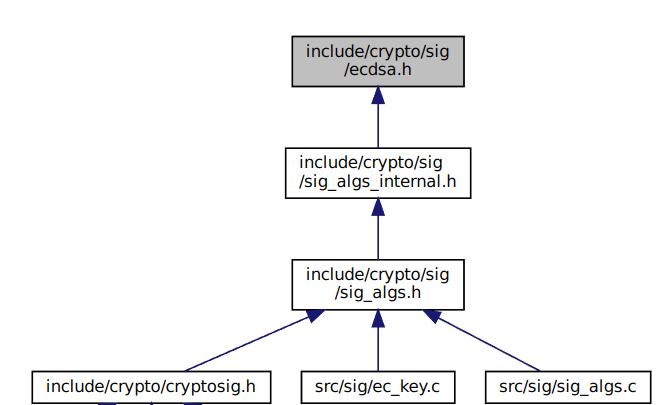
\includegraphics[scale=.7]{dep-graph/ecdsa.png}
\end{figure}

\newpage
\section{Build with Makefile}
This section describes the build system for generating (static) libraries, driven by a single GNU Makefile. It covers compiler settings, directory layout, source discovery, and all available targets.


\paragraph{Build without Makefile}\ \\
\begin{lstlisting}[numbers=none]
mkdir -p obj/nn obj/fp obj/utils
gcc -MMD -MP -c -O2 -std=c99 -Wall -Wextra -Iinclude -fPIC -o obj/nn/nn_add.o src/nn/nn_add.c
gcc -MMD -MP -c -O2 -std=c99 -Wall -Wextra -Iinclude -fPIC -o obj/nn/nn.o src/nn/nn.c
gcc -MMD -MP -c -O2 -std=c99 -Wall -Wextra -Iinclude -fPIC -o obj/nn/nn_div.o src/nn/nn_div.c
gcc -MMD -MP -c -O2 -std=c99 -Wall -Wextra -Iinclude -fPIC -o obj/nn/nn_logical.o src/nn/nn_logical.c
gcc -MMD -MP -c -O2 -std=c99 -Wall -Wextra -Iinclude -fPIC -o obj/nn/nn_modinv.o src/nn/nn_modinv.c
gcc -MMD -MP -c -O2 -std=c99 -Wall -Wextra -Iinclude -fPIC -o obj/nn/nn_mod_pow.o src/nn/nn_mod_pow.c
gcc -MMD -MP -c -O2 -std=c99 -Wall -Wextra -Iinclude -fPIC -o obj/nn/nn_mul.o src/nn/nn_mul.c
gcc -MMD -MP -c -O2 -std=c99 -Wall -Wextra -Iinclude -fPIC -o obj/nn/nn_mul_redc1.o src/nn/nn_mul_redc1.c
gcc -MMD -MP -c -O2 -std=c99 -Wall -Wextra -Iinclude -fPIC -o obj/nn/nn_rand.o src/nn/nn_rand.c

gcc -MMD -MP -c -O2 -std=c99 -Wall -Wextra -Iinclude -fPIC -o obj/fp/fp_add.o src/fp/fp_add.c
gcc -MMD -MP -c -O2 -std=c99 -Wall -Wextra -Iinclude -fPIC -o obj/fp/fp.o src/fp/fp.c
gcc -MMD -MP -c -O2 -std=c99 -Wall -Wextra -Iinclude -fPIC -o obj/fp/fp_mul.o src/fp/fp_mul.c
gcc -MMD -MP -c -O2 -std=c99 -Wall -Wextra -Iinclude -fPIC -o obj/fp/fp_mul_redc1.o src/fp/fp_mul_redc1.c
gcc -MMD -MP -c -O2 -std=c99 -Wall -Wextra -Iinclude -fPIC -o obj/fp/fp_pow.o src/fp/fp_pow.c
gcc -MMD -MP -c -O2 -std=c99 -Wall -Wextra -Iinclude -fPIC -o obj/fp/fp_rand.o src/fp/fp_rand.c
gcc -MMD -MP -c -O2 -std=c99 -Wall -Wextra -Iinclude -fPIC -o obj/fp/fp_sqrt.o src/fp/fp_sqrt.c

gcc -MMD -MP -c -O2 -std=c99 -Wall -Wextra -Iinclude -fPIC -o obj/utils/utils.o src/utils/utils.c
gcc -MMD -MP -c -O2 -std=c99 -Wall -Wextra -Iinclude -fPIC -o obj/utils/utils_rand.o src/utils/utils_rand.c
gcc -MMD -MP -c -O2 -std=c99 -Wall -Wextra -Iinclude -fPIC -o obj/utils/print_nn.o src/utils/print_nn.c
gcc -MMD -MP -c -O2 -std=c99 -Wall -Wextra -Iinclude -fPIC -o obj/utils/print_fp.o src/utils/print_fp.c
gcc -MMD -MP -c -O2 -std=c99 -Wall -Wextra -Iinclude -fPIC -o obj/utils/print_buf.o src/utils/print_buf.c

mkdir -p obj/external_deps
gcc -MMD -MP -c -O2 -std=c99 -Wall -Wextra -Iinclude -fPIC -o obj/external_deps/print.o src/external_deps/print.c
gcc -MMD -MP -c -O2 -std=c99 -Wall -Wextra -Iinclude -fPIC -o obj/external_deps/rand.o src/external_deps/rand.c
gcc -MMD -MP -c -O2 -std=c99 -Wall -Wextra -Iinclude -fPIC -o obj/external_deps/time.o src/external_deps/time.c

mkdir -p lib
ar rcs lib/libarith.a \
	obj/fp/fp_add.o obj/fp/fp.o obj/fp/fp_mul.o obj/fp/fp_mul_redc1.o obj/fp/fp_pow.o obj/fp/fp_rand.o obj/fp/fp_sqrt.o \
	obj/nn/nn_add.o obj/nn/nn.o obj/nn/nn_div.o obj/nn/nn_logical.o obj/nn/nn_modinv.o obj/nn/nn_mod_pow.o obj/nn/nn_mul.o obj/nn/nn_mul_redc1.o obj/nn/nn_rand.o \
	obj/utils/utils.o obj/utils/utils_rand.o obj/utils/print_nn.o obj/utils/print_fp.o obj/utils/print_buf.o \
	obj/external_deps/print.o obj/external_deps/rand.o obj/external_deps/time.o 

mkdir -p obj/curves
gcc -MMD -MP -c -O2 -std=c99 -Wall -Wextra -Iinclude -fPIC -o obj/curves/aff_pt.o src/curves/aff_pt.c
gcc -MMD -MP -c -O2 -std=c99 -Wall -Wextra -Iinclude -fPIC -o obj/curves/curves.o src/curves/curves.c
gcc -MMD -MP -c -O2 -std=c99 -Wall -Wextra -Iinclude -fPIC -o obj/curves/ec_params.o src/curves/ec_params.c
gcc -MMD -MP -c -O2 -std=c99 -Wall -Wextra -Iinclude -fPIC -o obj/curves/ec_shortw.o src/curves/ec_shortw.c
gcc -MMD -MP -c -O2 -std=c99 -Wall -Wextra -Iinclude -fPIC -o obj/curves/prj_pt.o src/curves/prj_pt.c
gcc -MMD -MP -c -O2 -std=c99 -Wall -Wextra -Iinclude -fPIC -o obj/utils/print_curves.o src/utils/print_curves.c

ar rcs lib/libec.a \
	obj/fp/fp_add.o obj/fp/fp.o obj/fp/fp_mul.o obj/fp/fp_mul_redc1.o obj/fp/fp_pow.o obj/fp/fp_rand.o obj/fp/fp_sqrt.o \
	obj/nn/nn_add.o obj/nn/nn.o obj/nn/nn_div.o obj/nn/nn_logical.o obj/nn/nn_modinv.o obj/nn/nn_mod_pow.o obj/nn/nn_mul.o obj/nn/nn_mul_redc1.o obj/nn/nn_rand.o \
	obj/utils/utils.o obj/utils/utils_rand.o obj/utils/print_nn.o obj/utils/print_fp.o obj/utils/print_buf.o \
	obj/curves/aff_pt.o obj/curves/curves.o obj/curves/ec_params.o obj/curves/ec_shortw.o obj/curves/prj_pt.o \
	obj/utils/print_curves.o \
	obj/external_deps/print.o obj/external_deps/rand.o obj/external_deps/time.o 

mkdir -p obj/hash obj/sig
gcc -MMD -MP -c -O2 -std=c99 -Wall -Wextra -Iinclude -fPIC -o obj/hash/sha256.o src/hash/sha256.c
gcc -MMD -MP -c -O2 -std=c99 -Wall -Wextra -Iinclude -fPIC -o obj/hash/sha3-256.o src/hash/sha3-256.c
gcc -MMD -MP -c -O2 -std=c99 -Wall -Wextra -Iinclude -fPIC -o obj/hash/sha3.o src/hash/sha3.c
gcc -MMD -MP -c -O2 -std=c99 -Wall -Wextra -Iinclude -fPIC -o obj/hash/shake256.o src/hash/shake256.c
gcc -MMD -MP -c -O2 -std=c99 -Wall -Wextra -Iinclude -fPIC -o obj/hash/shake.o src/hash/shake.c
gcc -MMD -MP -c -O2 -std=c99 -Wall -Wextra -Iinclude -fPIC -o obj/hash/hash_algs.o src/hash/hash_algs.c
gcc -MMD -MP -c -O2 -std=c99 -Wall -Wextra -Iinclude -fPIC -o obj/hash/hmac.o src/hash/hmac.c

gcc -MMD -MP -c -O2 -std=c99 -Wall -Wextra -Iinclude -fPIC -o obj/sig/ecdsa.o src/sig/ecdsa.c
gcc -MMD -MP -c -O2 -std=c99 -Wall -Wextra -Iinclude -fPIC -o obj/sig/ecdsa_common.o src/sig/ecdsa_common.c
gcc -MMD -MP -c -O2 -std=c99 -Wall -Wextra -Iinclude -fPIC -o obj/sig/sig_algs.o src/sig/sig_algs.c
gcc -MMD -MP -c -O2 -std=c99 -Wall -Wextra -Iinclude -fPIC -o obj/sig/ec_key.o src/sig/ec_key.c
gcc -MMD -MP -c -O2 -std=c99 -Wall -Wextra -Iinclude -fPIC -o obj/utils/print_keys.o src/utils/print_keys.c

ar rcs lib/libsign.a \
	obj/fp/fp_add.o obj/fp/fp.o obj/fp/fp_mul.o obj/fp/fp_mul_redc1.o obj/fp/fp_pow.o obj/fp/fp_rand.o obj/fp/fp_sqrt.o \
	obj/nn/nn_add.o obj/nn/nn.o obj/nn/nn_div.o obj/nn/nn_logical.o obj/nn/nn_modinv.o obj/nn/nn_mod_pow.o obj/nn/nn_mul.o obj/nn/nn_mul_redc1.o obj/nn/nn_rand.o \
	obj/utils/utils.o obj/utils/utils_rand.o obj/utils/print_nn.o obj/utils/print_fp.o obj/utils/print_buf.o \
	obj/curves/aff_pt.o obj/curves/curves.o obj/curves/ec_params.o obj/curves/ec_shortw.o obj/curves/prj_pt.o \
	obj/utils/print_curves.o \
	obj/hash/sha256.o obj/hash/sha3-256.o obj/hash/sha3.o obj/hash/shake256.o obj/hash/shake.o obj/hash/hash_algs.o obj/hash/hmac.o \
	obj/sig/ecdsa.o obj/sig/ecdsa_common.o obj/sig/sig_algs.o obj/sig/ec_key.o \
	obj/utils/print_keys.o \
	obj/external_deps/print.o obj/external_deps/rand.o obj/external_deps/time.o 
\end{lstlisting}

\newpage
\paragraph{Build with Makefile}\ \\
\ \\
\textbf{[gcc (GNU Compiler Collection)]}
\begin{itemize}
	\item \texttt{gcc}: compiles and links source code.
\end{itemize}
\textbf{[ar \texttt{rcs} (GNU Archiver)]}
\begin{itemize}
	\item \texttt{ar rcs}: creates or updates static library archives.
	\begin{itemize}
		\item \texttt{r}: ``replace'' -- add or replace files in the archive.
		\item \texttt{c}: ``create'' -- silently create the archive if it doesn’t exist.
		\item \texttt{s}: ``index'' -- write an index (symbol table) for faster linking.
	\end{itemize}
	Creates and maintains static library archives (\texttt{.a}) from object files.
\end{itemize}

\begin{lstlisting}[numbers=none]
#-------------------------------------------------------------------------------
# Makefile: separate obj/, lib/, bin/; builds libarith.a, libec.a, libsign.a
#-------------------------------------------------------------------------------

# Directories
OBJ_DIR   := obj
LIB_DIR   := lib
BIN_DIR   := bin
INCLUDE   := include
SRC_DIR   := src

# Compiler & tools
CC        := gcc
AR        := ar rcs

# Flags
CFLAGS    := -MMD -MP -O3 -std=c99 -Wall -Wextra -I$(INCLUDE)
PICFLAGS  := -fPIC

# Module source files
FP_SRCS      := $(wildcard $(SRC_DIR)/fp/fp_*.c)
NN_SRCS      := $(wildcard $(SRC_DIR)/nn/nn_*.c) $(SRC_DIR)/nn/nn.c
UTILS_ARITH  := $(SRC_DIR)/utils/utils.c $(SRC_DIR)/utils/utils_rand.c
UTILS_PRINT  := $(wildcard $(SRC_DIR)/utils/print_*.c)
CURVES_SRCS  := $(wildcard $(SRC_DIR)/curves/*.c)
HASH_SRCS    := $(wildcard $(SRC_DIR)/hash/*.c)
SIG_SRCS     := $(SRC_DIR)/sig/ecdsa.c $(SRC_DIR)/sig/ecdsa_common.c $(SRC_DIR)/sig/sig_algs.c $(SRC_DIR)/sig/ec_key.c

# Generate object lists by mirroring src/ to obj/
define to_obj
	$(patsubst $(SRC_DIR)/%, $(OBJ_DIR)/%, $(1:.c=.o))
endef

FP_OBJS       := $(call to_obj,$(FP_SRCS))
NN_OBJS       := $(call to_obj,$(NN_SRCS))
UTILS_ARITH_OBJS := $(call to_obj,$(UTILS_ARITH))
UTILS_PRINT_OBJS := $(call to_obj,$(UTILS_PRINT))
CURVES_OBJS   := $(call to_obj,$(CURVES_SRCS))
HASH_OBJS     := $(call to_obj,$(HASH_SRCS))
SIG_OBJS      := $(call to_obj,$(SIG_SRCS))

# Library object groups
LIBARITH_OBJS := $(FP_OBJS) $(NN_OBJS) $(UTILS_ARITH_OBJS) $(UTILS_PRINT_OBJS)
LIBEC_OBJS    := $(LIBARITH_OBJS) $(CURVES_OBJS)
LIBSIGN_OBJS  := $(LIBEC_OBJS) $(HASH_OBJS) $(SIG_OBJS)

# All objects and deps
ALL_OBJS      := $(sort $(LIBSIGN_OBJS))
DEPS          := $(ALL_OBJS:.o=.d)

# Phony targets
.PHONY: all clean rebuild
all: $(LIB_DIR)/libarith.a $(LIB_DIR)/libec.a $(LIB_DIR)/libsign.a

clean:
	rm -rf $(OBJ_DIR) $(LIB_DIR) $(BIN_DIR)
	rm -f *~

# Compile rule: .c => .o (+ deps)
$(OBJ_DIR)/%.o: $(SRC_DIR)/%.c
	@mkdir -p $(dir $@)
	$(CC) $(CFLAGS) $(PICFLAGS) -MMD -MP -c $< -o $@

# Static libraries
$(LIB_DIR)/libarith.a: $(LIBARITH_OBJS)
	@mkdir -p $(LIB_DIR)
	$(AR) $@ $^

$(LIB_DIR)/libec.a: $(LIBEC_OBJS)
	@mkdir -p $(LIB_DIR)
	$(AR) $@ $^

$(LIB_DIR)/libsign.a: $(LIBSIGN_OBJS)
	@mkdir -p $(LIB_DIR)
	$(AR) $@ $^

rebuild:
	$(MAKE) clean
	$(MAKE) -j8

# Include dependency files
-include $(DEPS)
\end{lstlisting}
%\paragraph{Common \texttt{gcc} Options}
\begin{itemize}
	\item \texttt{-MMD}: generates dependency files (\texttt{.d}) for user headers
	\item \texttt{-MP}: adds phony targets for missing headers.
	\item \texttt{-O3}: enables high-level optimizations.
	\item \texttt{-std=c99}: enforces ISO C99 compliance.
	\item \texttt{-Wall}: enables a broad set of common warning checks to catch potential issues early.
	\item \texttt{-Wextra}: enables additional, more pedantic warnings beyond \texttt{-Wall}.
	\item \texttt{-Iinclude}: adds the \texttt{include/} directory to the header search path.
	\item \texttt{-fPIC}: generates position-independent code for use in shared libraries, allowing flexible load addresses.
\end{itemize}
\begin{lstlisting}[numbers=none]
@:~$ cd lib
@:~$ ls -lh 
total 552K
-rw-rw-r-- 1 hacker-code-j hacker-code-j 123K Jun 11 06:58 libarith.a
-rw-rw-r-- 1 hacker-code-j hacker-code-j 176K Jun 11 06:58 libec.a
-rw-rw-r-- 1 hacker-code-j hacker-code-j 251K Jun 11 06:58 libsign.a
\end{lstlisting}
\newpage
\section{Sample Code}
\begin{lstlisting}[style=cstyle,caption={sample\_ecdsa.c},captionpos=t]
/* 
 * sample_ecdsa.c
 * 
 * A minimal example of using libecc’s ECDSA on NIST P-256 to sign and verify
 * a simple message string.
 */

#include <stdio.h>
#include <stdlib.h>
#include <string.h>
#include <fcntl.h>
#include <unistd.h>
#include <stdint.h>

#include <crypto/cryptosig.h> // For ECDSA

// Hex-encode buffer
static char *to_hex(const uint8_t *buf, size_t len) {
	static const char hex[] = "0123456789ABCDEF";
	char *out = malloc(len*2 + 1);
	for (size_t i = 0; i < len; i++) {
		out[2*i]   = hex[buf[i] >> 4];
		out[2*i+1] = hex[buf[i] & 0xF];
	}
	out[len*2] = '\0';
	return out;
}

int main(void) {
	// 1. Load P-256 parameters
	ec_params params;
	import_params(&params, &secp256r1_str_params);
	
	// 2. Generate key pair
	ec_key_pair kp;
	if (ec_key_pair_gen(&kp, &params, ECDSA) != 0) {
		fprintf(stderr, "Key generation failed\n");
		return 1;
	}
	
	// 3. Prepare message and hash it
	const char *msg = "Hello, ECDSA!";
	const hash_mapping *hm;
	if (get_hash_by_type(SHA256, &hm) != 0) {
		fprintf(stderr, "SHA-256 not available\n");
		return 1;
	}
	hash_context hctx;
	hm->hfunc_init(&hctx);
	hm->hfunc_update(&hctx, (const uint8_t*)msg, (u32)strlen(msg));
	uint8_t digest[64];
	u8 dlen = hm->digest_size;
	hm->hfunc_finalize(&hctx, digest);
	
	// 4. Sign the digest
	u8 siglen;
	ec_get_sig_len(&params, ECDSA, SHA256, &siglen);
	uint8_t *sigbin = malloc(siglen);
	if (ec_sign(sigbin, siglen,
	&kp, digest, dlen,
	ECDSA, SHA256,
	NULL, 0) != 0)
	{
		fprintf(stderr, "Signing failed\n");
		free(sigbin);
		return 1;
	}
	
	char *hexsig = to_hex(sigbin, siglen);
	printf("Signature: %s\n", hexsig);
	
	// 5. Derive public key and verify
	ec_pub_key pub;
	if (init_pubkey_from_privkey(&pub, &kp.priv_key) != 0) {
		fprintf(stderr, "Public key derivation failed\n");
		free(sigbin);
		free(hexsig);
		return 1;
	}
	
	int ok = ec_verify(sigbin, siglen,
	&pub, digest, dlen,
	ECDSA, SHA256,
	NULL, 0);
	printf("Verification: %s\n", (ok == 0) ? "SUCCESS" : "FAILURE");
	
	// Cleanup
	free(sigbin);
	free(hexsig);
	return (ok == 0) ? 0 : 1;
}
\end{lstlisting}
\begin{lstlisting}[numbers=none]
@:~$ gcc -std=c99 -D_POSIX_C_SOURCE=200809L -O2 -Iinclude \
	sample_ecdsa.c -o sample_ecdsa \
	lib/libarith.a lib/libec.a lib/libsign.a
@:~$ ./sample_ecdsa   
Signature:  0934EE14D27FB767668EE5EA1E850165B47C0624D34B74D53E77846FE868A042A036D3AA4E2C67EB1
F8EE2F6948C68378CF88E2E04CB48EB63CEA78AE4D14FF9
Verification: SUCCESS
\end{lstlisting}